%
% File naaclhlt2010.tex
%
% Contact: nasmith@cs.cmu.edu

\documentclass[11pt,letterpaper]{article}
\usepackage{naaclhlt2010}
\usepackage{times}
\usepackage{latexsym}
\usepackage{hyperref}
\usepackage{graphicx}
\usepackage{wrapfig}
\usepackage{url}
\usepackage{wrapfig}
\usepackage{color}
\usepackage{marvosym}
\usepackage{enumerate}
\usepackage{subfigure}
\usepackage{tikz}
\usepackage{amsmath}
\usepackage{amssymb}
\usepackage{hyperref}
\usepackage{bbm}

\DeclareMathOperator*{\argmax}{arg\,max}

\setlength\titlebox{4cm}    % Expanding the titlebox


\newcommand{\vwi}{{\bf w}_i}
\newcommand{\vw}{{\bf w}}
\newcommand{\vx}{{\bf x}}
\newcommand{\vy}{{\bf y}}
\newcommand{\vb}{{\bf b}}
\newcommand{\valpha}{{\bf \alpha}}
\newcommand{\vxi}{{\bf x}_i}
\newcommand{\yi}{y_i}
\newcommand{\vxj}{{\bf x}_j}
\newcommand{\vxn}{{\bf x}_n}
\newcommand{\yj}{y_j}
\newcommand{\ai}{\alpha_i}
\newcommand{\aj}{\alpha_j}
\newcommand{\X}{{\bf X}}
\newcommand{\Y}{{\bf Y}}
\newcommand{\vz}{{\bf z}}
\newcommand{\msigma}{{\bf \Sigma}}
\newcommand{\vmu}{{\bf \mu}}
\newcommand{\vmuk}{{\bf \mu}_k}
\newcommand{\msigmak}{{\bf \Sigma}_k}
\newcommand{\vmuj}{{\bf \mu}_j}
\newcommand{\msigmaj}{{\bf \Sigma}_j}
\newcommand{\pij}{\pi_j}
\newcommand{\pik}{\pi_k}
\newcommand{\D}{\mathcal{D}}
\newcommand{\el}{\mathcal{L}}
\newcommand{\N}{\mathcal{N}}
\newcommand{\vxij}{{\bf x}_{ij}}
\newcommand{\vt}{{\bf t}}
\newcommand{\yh}{\hat{y}}
\newcommand{\code}[1]{{\footnotesize \tt #1}}
\newcommand{\alphai}{\alpha_i}

\title{2D Visualizations for Support Vector Machine and Neural Network}

\author{Jizhou Xu \, Aileme Omogbai \\
	Johns Hopkins University \\
	{\tt $\{jxu55, aomogba1\}$@jhu.edu}}

\date{December 10, 2014}

\begin{document}
\maketitle
\begin{abstract}
We present a web-based demo that helps to visualize the operations and results of some machine learning binary classification algorithms. For this project, we have chosen to implement two non-linear methods, namely Support Vector Machines (SVM) and Artificial Neural Networks. This visualization tool is implemented fully in Javascript and so the data collection,  training  and display of the results is done on the client-side. It displays a 2D canvas such that data points can be added with mouse clicks and the decision boundary generated by the algorithm is displayed. The data points correspond to the $(x,y)$ positions of the points clicked on the canvas. There is also provision for adjusting some parameters of the model. The visualization can be found at \url{http://metoerite-j.github.io/Visual-Machine-Learning}.
\end{abstract}

\section{Introduction}

In the field of machine learning, binary classification problems stem from the need to separate a set of data points into two different classes. In the supervised case, we have data that is already separated such that each data point belongs to one of the defined classes. For the unsupervised case, we do not know the classes for the example data available. In both cases, we wish to find a model that can learn parameters for the classification such that new unlabeled data points can be assigned to the right class. The model therefore creates "boundaries" such that a data point is labeled according to the side of the boundary that it falls in. 

If the boundary used to separate the two sets of data points is a line, then the problem is a linear classification problem. The data is not usually linearly separable and so complex functions may be needed to define the boundary. Also, while it is intuitive to visualize the concept of the boundary in 2 dimensions, the data is usually of much higher dimensions. This means that very complex decision boundaries are needed to bring about separation in practical applications. Even in 2D however, it may be difficult to picture the boundary that is generated by non-linear classifiers, and that is what this project aims to help with.

We present a web visualization tool that shows the classification results of two popular non-linear classifiers. The user is presented with a 2D canvas that contains default points that have been generated with a normal distribution and classified randomly. The classes used for the demo are represented by the colors black/white and this used to label the data points and the regions on the canvas. So, a point is labeled either black or white. Also, the color of any position in the canvas represents the class that a test data point (i.e. a point we want to classify) will be assigned to by the current model. Therefore, the boundary between the white and black regions on the canvas represent the decision boundary that was generated by the algorithm used. 

At the current stage, we have implemented two popular non-linear classifiers: Support Vector Machines (SVM) and Artificial Neural Network (ANN). For training the SVM, we used the Primal Estimated Sub-Gradient Solver for SVM (Pegasos) algorithm. For neural networks training, we used the feed-forward back-propagation neural network as our model. 
SVMs are effective and popular classification learning tool. The task of learning a support vector machine is cast as a constrained quadratic programming problem.  stochastic sub-gradians descent algorithm for solving the optimization problem cast by SVMs.

\begin{figure*}
\centering
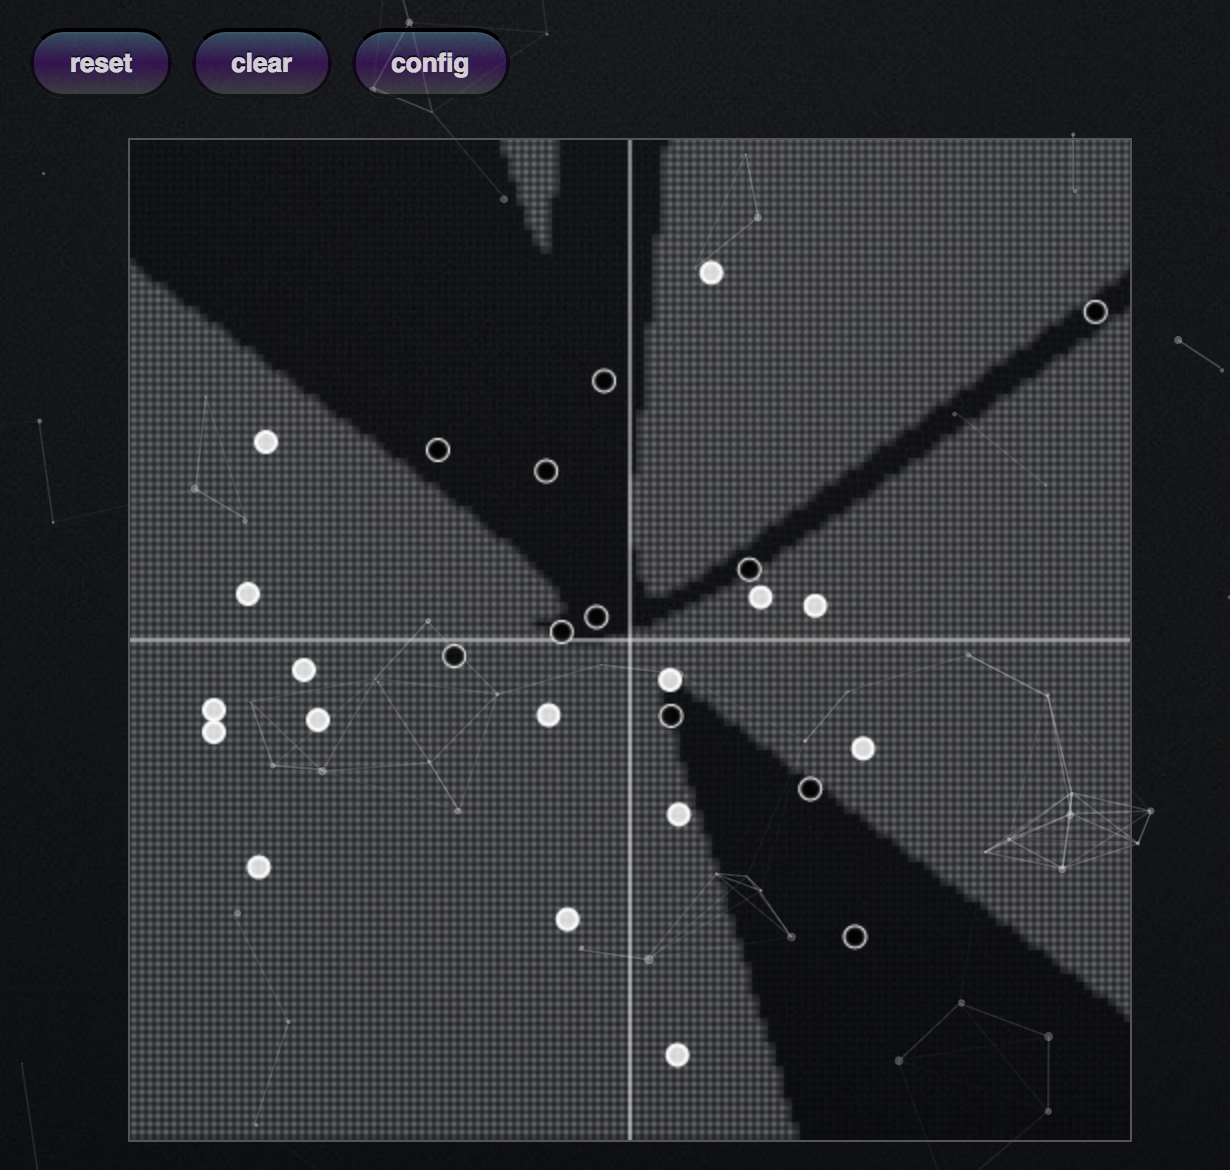
\includegraphics[scale=.5]{images/Intro.PNG}
\caption{Sample output}
\label{fig:intro}
\end{figure*}

\section{SVM}

\subsection{Background}
	The SVM is a very popular model for classification. In the SVM model, data points are seen as points in the $m$-dimensional plane defined by the data. The intuition is that we want to separate the data points with an $(m-1)$-dimensional hyperplane which corresponds to a linear separation. We want to choose the separating line such that its distance to the nearest data point on each side is maximized, which is called maximizing the margin. So we learn the weights in each dimension for that hyperplane. The data points that are closest to the separating hyperplane, that is the data points that affect the position of the hyperplane are called the support vectors. Formally, given a training set $\{(\vxi,\yi)\}_{i=1}^N$, where $\vx_i \in \mathbb{R}^M$ and $y_i \in\{+1,-1\}$, we want to solve the constrained the problem:
\begin{align}
\argmax_{\valpha >= 0} \min_{\vw,b} \{ \frac{1}{2} ||w||^2  - \sum_i^N \alpha_i\left[\yi(\vw \vx - b) - 1\right]  \}
\end{align}
where $b$ is the bias term that determines the offset of the hyperplane from the origin, $w$ denotes the normal vector to the hyperplane and $\alpha$ are Lagrange multipliers. This equation is known as the primal formulation of the optimization problem.

What makes SVMs very popular is that they can be made into non-linear classifiers by applying the "kernel trick". The algorithm is essentially the same except that the dot product used to compute the margins is replaced with a kernel function that represents a dot product also, but in a higher dimension. In this project, we used the radial basis function (RBF) kernel to separate non-linearly separable data.

%\begin{figure*}
%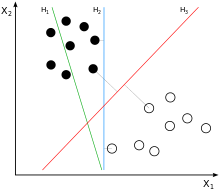
\includegraphics[scale=1]{images/Svm_separating_hyperplanes.PNG}
%\caption{SVM margins [Wikipedia]}
%\label{fig:svm}
%\end{figure*}
\subsection{Training}
There are different algorithms for training SVMs like:
\begin{enumerate}
\item
the Sequential Minimal Optimization (SMO), and
\item
Primal Estimated sub-GrAdient SOlver for SVM (Pegasos).
\end{enumerate} 

We chose to implement the Pegasos algorithm for training the SVM in this project. The basic algorithm involves using stochastic gradient descent to solve the primal formulation of the problem in $w$ which corresponds to the linear SVM. However, as explained  in $•$, the algorithm can also be modified to handle the non-linear kernelized case as well. See the paper for more information on the algorithm. We have implemented both versions of the algorithm, so the user can try both the linear and kernel forms to see the boundaries generated by each model type. The application also makes it possible for the user to generate synthetic linearly separable data in order to see the linear SVM solution better. 

\subsection{Implementation}
The implementation of the SVM visualization is divided into two sections. This applies to the other models as well. The actual implementation of the Pegasos algorithm is in a js file that is separate from the actual visualization page. That file thus contains the code for training the SVM, predicting the class of points after training and all other functions necessary for the training algorithm to work. The usage is as follows:
\begin{enumerate}[i]
\item
Create a new instance of the Pegasos trainer: $pegasos.SVM$.
\item
Call the $train$ method, passing in the data points, the labels and the options for training. Some of the options include: the value of $\lambda$ used in the Pegasos algorithm, number of iterations to be run, the type of kernel ("linear" for linear SVM, and for now "rbf" for RBF kernel), and the value of $\sigma$ for the RBF kernel.
\item
After training, call $predictOne$ to predict a specific data point, or $predict$ for a set of points.
\end{enumerate}
The linear and kernelized versions of the Pegasos are quite different and so they are implemented separately and used depending on which is specified in the training options. For the linear case, the model parameters are the $w$ values but in the kernelized version, its easier to keep the parameters as $\alpha$, the Lagrangian multipliers. These values are used to predict the class of points after training.

The visualization page calls the training algorithm and displays the results on the canvas. Once the page is loaded, default data points corresponding to points on the canvas are generated from a Gaussian distribution and classified arbitrarily. The data is used to train the model. For drawing the data points, boundaries and many finicky details of 2D drawing with Javascript, we made use of a library written by Andrej Karpathy $•$. To display the decision boundary, we predict the class of every point on the canvas. The boundary is seen as the separation between the white and dark regions on the canvas.

The user is able to switch from a linear SVM to using a kernel and the model is retrained appropriately and the decision boundary displayed. For the linear SVM, we show the decision boundary and the margins of the classifier. Because the default data generated is not likely to be linearly separable, we provided an option to clear the points and input new data points. This can be used to generate linearly separable data, because the linear classifier will not produce sensible boundaries for non-linear data.

It is also possible to vary the value of the parameter of the RBF kernel $\sigma$, which has a big effect on the shape of the decision boundary. By the definition of the kernel, small values of $\sigma$ will make it such that only points close to each other will affect prediction because the value of the kernel will be close to zero for points far from each other. The model will look to be overfitting the data. For large values of $\sigma$, we get smooth boundaries that mis-classifies points, tending towards a linear classifier.

\subsection{Results}


\subsection{The SMO Algorithm}
\label{sect:pdf}

For the production of the electronic manuscript you must use Adobe's
Portable Document Format (PDF). This format can be generated from
postscript files: on Unix systems, you can use {\tt ps2pdf} for this
purpose; under Microsoft Windows, you can use Adobe's Distiller, or
if you have cygwin installed, you can use {\tt dvipdf} or
{\tt ps2pdf}.  Note 
that some word processing programs generate PDF which may not include
all the necessary fonts (esp. tree diagrams, symbols). When you print
or create the PDF file, there is usually an option in your printer
setup to include none, all or just non-standard fonts.  Please make
sure that you select the option of including ALL the fonts.  {\em
  Before sending it, test your {\/\em PDF} by printing it from a
  computer different from the one where it was created}. Moreover,
some word processor may generate very large postscript/PDF files,
where each page is rendered as an image. Such images may reproduce
poorly.  In this case, try alternative ways to obtain the postscript
and/or PDF.  One way on some systems is to install a driver for a
postscript printer, send your document to the printer specifying
``Output to a file'', then convert the file to PDF.

For reasons of uniformity, Adobe's {\bf Times Roman} font should be
used. In \LaTeX2e{} this is accomplished by putting

\begin{quote}
\begin{verbatim}
\usepackage{times}
\usepackage{latexsym}
\end{verbatim}
\end{quote}
in the preamble.

Additionally, it is of utmost importance to specify the {\bf
  US-Letter format} (8.5in $\times$ 11in) when formatting the paper.
When working with {\tt dvips}, for instance, one should specify {\tt
  -t letter}.

Print-outs of the PDF file on US-Letter paper should be identical to the
hardcopy version.  If you cannot meet the above requirements about the
production of your electronic submission, please contact the
publication chairs above  as soon as possible.


\subsection{Layout}
\label{ssec:layout}

Format manuscripts two columns to a page, in the manner these
instructions are formatted. The exact dimensions for a page on US-letter
paper are:

\begin{itemize}
\item Left and right margins: 1in
\item Top margin:1in
\item Bottom margin: 1in
\item Column width: 3.15in
\item Column height: 9in
\item Gap between columns: 0.2in
\end{itemize}

\noindent Papers should not be submitted on any other paper size. Exceptionally,
authors for whom it is \emph{impossible} to format on US-Letter paper,
may format for \emph{A4} paper. In this case, they should keep the \emph{top}
and \emph{left} margins as given above, use the same column width,
height and gap, and modify the bottom and right margins as necessary.
Note that the text will no longer be centered.

\subsection{How We Implemented it}
\label{ssec:first}

Center the title, author's name(s) and affiliation(s) across both
columns. Do not use footnotes for affiliations.  Do not include the
paper ID number assigned during the submission process. 
Use the two-column format only when you begin the abstract.

{\bf Title}: Place the title centered at the top of the first page, in
a 15 point bold font.  (For a complete guide to font sizes and styles, see Table~\ref{font-table}.)
Long title should be typed on two lines without
a blank line intervening. Approximately, put the title at 1in from the
top of the page, followed by a blank line, then the author's names(s),
and the affiliation on the following line.  Do not use only initials
for given names (middle initials are allowed). Do not format surnames
in all capitals (e.g., ``Leacock,'' not ``LEACOCK'').  The affiliation should
contain the author's complete address, and if possible an electronic
mail address. Leave about 0.75in between the affiliation and the body
of the first page.

{\bf Abstract}: Type the abstract at the beginning of the first
column.  The width of the abstract text should be smaller than the
width of the columns for the text in the body of the paper by about
0.25in on each side.  Center the word {\bf Abstract} in a 12 point
bold font above the body of the abstract. The abstract should be a
concise summary of the general thesis and conclusions of the paper.
It should be no longer than 200 words.  The abstract text should be in 10 point font.

{\bf Text}: Begin typing the main body of the text immediately after
the abstract, observing the two-column format as shown in 
the present document.  Do not include page numbers.

{\bf Indent} when starting a new paragraph. For reasons of uniformity,
use Adobe's {\bf Times Roman} fonts, with 11 points for text and 
subsection headings, 12 points for section headings and 15 points for
the title.  If Times Roman is unavailable, use {\bf Computer Modern
  Roman} (\LaTeX2e{}'s default; see section \ref{sect:pdf} above).
Note that the latter is about 10\% less dense than Adobe's Times Roman
font.

\subsection{Sections}

{\bf Headings}: Type and label section and subsection headings in the
style shown on the present document.  Use numbered sections (Arabic
numerals) in order to facilitate cross references. Number subsections
with the section number and the subsection number separated by a dot,
in Arabic numerals. 

{\bf Citations}: Citations within the text appear
in parentheses as~\cite{Gusfield:97} or, if the author's name appears in
the text itself, as Gusfield~\shortcite{Gusfield:97}. 
Append lowercase letters to the year in cases of ambiguities.  
Treat double authors as in~\cite{Aho:72}, but write as 
in~\cite{Chandra:81} when more than two authors are involved. 
Collapse multiple citations as in~\cite{Gusfield:97,Aho:72}.

\textbf{References}: Gather the full set of references together under
the heading {\bf References}; place the section before any Appendices,
unless they contain references. Arrange the references alphabetically
by first author, rather than by order of occurrence in the text.
Provide as complete a citation as possible, using a consistent format,
such as the one for {\em Computational Linguistics\/} or the one in the 
{\em Publication Manual of the American 
Psychological Association\/}~\cite{APA:83}.  Use of full names for
authors rather than initials is preferred.  A list of abbreviations
for common computer science journals can be found in the ACM 
{\em Computing Reviews\/}~\cite{ACM:83}.

The \LaTeX{} and Bib\TeX{} style files provided roughly fit the
American Psychological Association format, allowing regular citations, 
short citations and multiple citations as described above.

{\bf Appendices}: Appendices, if any, directly follow the text and the
references (but see above).  Letter them in sequence and provide an
informative title: {\bf Appendix A. Title of Appendix}.

\textbf{Acknowledgment} sections should go as a last (unnumbered) section immediately
before the references.  

\subsection{Footnotes}

{\bf Footnotes}: Put footnotes at the bottom of the page. They may
be numbered or referred to by asterisks or other
symbols.\footnote{This is how a footnote should appear.} Footnotes
should be separated from the text by a line.\footnote{Note the
line separating the footnotes from the text.}  Footnotes should be in 9 point font.

\subsection{Graphics}

{\bf Illustrations}: Place figures, tables, and photographs in the
paper near where they are first discussed, rather than at the end, if
possible.  Wide illustrations may run across both columns and should be placed at
the top of a page. Color illustrations are discouraged, unless you have verified that 
they will be understandable when printed in black ink.

\begin{table}
\begin{center}
\begin{tabular}{|l|rl|}
\hline \bf Type of Text & \bf Font Size & \bf Style \\ \hline
paper title & 15 pt & bold \\
author names & 12 pt & bold \\
author affiliation & 12 pt & \\
the word ``Abstract'' & 12 pt & bold \\
section titles & 12 pt & bold \\
document text & 11 pt  &\\
abstract text & 10 pt & \\
captions & 10 pt & \\
bibliography & 10 pt & \\
footnotes & 9 pt & \\
\hline
\end{tabular}
\end{center}
\caption{\label{font-table} Font guide. }
\end{table}

{\bf Captions}: Provide a caption for every illustration; number each one
sequentially in the form:  ``Figure 1. Caption of the Figure.'' ``Table 1.
Caption of the Table.''  Type the captions of the figures and 
tables below the body, using 10 point text.  

\section{Length of Submission}
\label{sec:length}

The NAACL HLT 2010 main conference accepts submissions of long papers
and short papers.  The maximum length of a long paper manuscript is
eight (8) pages of content and one (1) additional page of references
\emph{only} (appendices count against the eight pages, not the
additional one page).  The maximum length of a short paper manuscript
is four (4) pages including references.  For both long and short
papers, all illustrations, references, and appendices must be
accommodated within these page limits, observing the formatting
instructions given in the present document.  Papers that do not
conform to the specified length and formatting requirements are
subject to be rejected without review.

% Up to two (2) additional pages may be purchased from ACL at the
% price of \$250 per page; please contact the publication chairs above
% for more information about this option.

\section*{Acknowledgments}

Do not number the acknowledgment section.

\begin{thebibliography}{}

\bibitem[\protect\citename{Aho and Ullman}1972]{Aho:72}
Alfred~V. Aho and Jeffrey~D. Ullman.
\newblock 1972.
\newblock {\em The Theory of Parsing, Translation and Compiling}, volume~1.
\newblock Prentice-{Hall}, Englewood Cliffs, NJ.

\bibitem[\protect\citename{{American Psychological Association}}1983]{APA:83}
{American Psychological Association}.
\newblock 1983.
\newblock {\em Publications Manual}.
\newblock American Psychological Association, Washington, DC.

\bibitem[\protect\citename{{Association for Computing Machinery}}1983]{ACM:83}
{Association for Computing Machinery}.
\newblock 1983.
\newblock {\em Computing Reviews}, 24(11):503--512.

\bibitem[\protect\citename{Chandra \bgroup et al.\egroup }1981]{Chandra:81}
Ashok~K. Chandra, Dexter~C. Kozen, and Larry~J. Stockmeyer.
\newblock 1981.
\newblock Alternation.
\newblock {\em Journal of the Association for Computing Machinery},
  28(1):114--133.

\bibitem[\protect\citename{Gusfield}1997]{Gusfield:97}
Dan Gusfield.
\newblock 1997.
\newblock {\em Algorithms on Strings, Trees and Sequences}.
\newblock Cambridge University Press, Cambridge, UK.

\end{thebibliography}

\end{document}
